
\def\thesislang{english} %change this depending on your language
\author{Gudeta Gebremariam}
\def\thesis{Thesis}
\def\alaotsikko{}

%Finnish section
\def\otsikko{Opinnäytetyön otsikko}
\def\tutkinto{Tutkinto}
\def\kohjelma{Koulutusohjelma}
\def\suuntautumis{Suuntautumisvaihtoehto}
\def\ohjaajat{
Olli Hämäläinen, Lehtori
}
\def\avainsanat{avainsanat}
\def\pvm{\ddmmyyyydate\today}

%English section, for abstract
\title{Speech synthesis }
\def\metropoliadegree {Bachelor of Engineering}
\def\metropoliadegreeprogramme {Information Technology}
\def\metropoliaspecialisation {Software Engineering}
\def\metropoliainstructors {
%Gudeta Gebremariam, Title (for example: Project Manager)\newline
Olli Hämäläinen, Senior Lecturer 
}
\def\metropoliakeywords {Language, Speech Synthesis, Speech, Web application}
\date{\today}

%----------------------------------------------------------------------------------------
%	GLOBAL STYLES
%----------------------------------------------------------------------------------------


\documentclass[11pt,a4paper,oneside,article]{memoir}


\usepackage{cmap} %make text searchable
\usepackage[T2A]{fontenc}

\usepackage[\thesislang]{babel} 
\usepackage{iflang}
\usepackage{amsmath}
\usepackage{amsfonts}
\usepackage{amssymb}
\usepackage{fontspec}
\usepackage{tocloft}
\usepackage{titlesec}
\usepackage[hyphens]{url}
\usepackage{mathtools}
\usepackage{wallpaper}
\usepackage{datetime}
\usepackage{listings}
\usepackage{color}
\usepackage[bookmarksdepth=subsection]{hyperref} % for automagic pdf links for toc, refs, etc.
\usepackage[amssymb]{SIunits}
\usepackage[version=3]{mhchem}
\usepackage{pgfplots} %simple plots etc
\usepackage{pgfplotstable}
\usepackage{tikz} % mindmaps, flowcharts, piecharts, examples at http://www.texample.net/tikz/examples/
\usetikzlibrary{shapes.geometric, arrows}


\renewcommand{\dateseparator}{.}
%condition for adding or not space in TOC
\usepackage{etoolbox}
%for compact list
\usepackage{enumitem}
%for block comment
\usepackage{verbatim}
%for "easier" references
\usepackage{varioref}
%forcing single line spacing in bibliography
\DisemulatePackage{setspace}
\usepackage{setspace}
%including figure (image)
\usepackage{graphicx}
%change the numbering for figure
\usepackage{chngcntr}
%strike trough
\usepackage{ulem}
%euro symbol
\usepackage{eurosym}
%try to count
\usepackage{totcount}
%insert source code
\usepackage{listings}
\usepackage[justification=justified,singlelinecheck=false]{caption}
\usepackage{color}
%force the width of a table instead of column
\usepackage{tabularx}
\usepackage{booktabs} %why not booktabs? :3

\newcommand\tn[1]{\textnormal{#1}} %use \tn instead of \textnormal
\newcommand\reaction[1]{\begin{equation}\ce{#1}\end{equation}} %\reaction{} for chemical reactions

%NORMAL TEXT
%all text, title, etc. in the same font: Arial
%replace with arial.ttf if you have the fontfile
%NOTE: fontname is case-sensitive
\setmainfont
[BoldFont=LiberationSans-Bold.ttf,
ItalicFont=LiberationSans-Italic.ttf,
BoldItalicFont=LiberationSans-BoldItalic.ttf]
{LiberationSans-Regular.ttf}
%line space
\linespread{1.5}
%\doublespacing
%margin
\usepackage[top=2.5cm, bottom=3cm, left=4cm, right=2cm, nofoot]{geometry}
\setlength{\parindent}{0pt} %first line of paragraph not indented
\setlength{\parskip}{16.5pt} %one empty line to separate paragraph
%list with small line space separation
\tightlists

%IMAGE - FIGURE
%the figures should be placed in the "illustration" folder
\graphicspath{{illustration/}}
%figure number without chapter (1.1, 1.2, 2.1) to (1, 2, 3)
\counterwithout{figure}{chapter}
%border around images
\setlength\fboxsep{0pt}
\setlength\fboxrule{0.5pt}
%caption font size
\captionnamefont{\small}
\captiontitlefont{\small}
%space after figure caption (and other float elements)
\setlength{\belowcaptionskip}{-7pt}

%TABLE
\counterwithout{table}{chapter}

%SOURCE CODE
\definecolor{darkgray}{rgb}{.4,.4,.4}
\definecolor{purple}{rgb}{0.65, 0.12, 0.82}
\lstset{
extendedchars=true,
captionpos=b,
caption=\footnotesize,
basicstyle=\singlespacing\ttfamily,%\small\fontfamily{"Courier"}\selectfont,
keywordstyle=\color{blue}\bfseries,
commentstyle=\color{purple}\itshape,
identifierstyle=\color{black},
stringstyle=\color{red},
showstringspaces=false,
showspaces=false,
numbers=left,
numberstyle=\footnotesize,
numbersep=9pt,
breaklines=true,
tabsize=2,
showtabs=false,
xleftmargin=1cm
}
\IfLanguageName {finnish} {\renewcommand{\lstlistingname}{Listaus}} {} % what is a good translation for this?
%\counterwithout{lstlisting}{chapter}
%moved after begin document, otherwise does not compile

%TOC
%change toc title
\IfLanguageName {finnish} {\addto{\captionsfinnish}{\renewcommand*{\contentsname}{Sisällys}}} {}
%remove dots
\renewcommand*{\cftdotsep}{\cftnodots}
%chapter title and page number not in bold
\renewcommand{\cftchapterfont}{}
\renewcommand{\cftchapterpagefont}{}
%sub section in toc
\setcounter{tocdepth}{2}
%subsection numbered
\setcounter{secnumdepth}{2}
\renewcommand{\tocheadstart}{\vspace*{-15pt}}
\renewcommand{\printtoctitle}[1]{\fontsize{13pt}{13pt}\bfseries #1}
\renewcommand{\aftertoctitle}{\vspace*{-22pt}\afterchaptertitle}
%spacing afer a chapter in toc
\preto\section{%
  \ifnum\value{section}=0\addtocontents{toc}{\vskip11pt}\fi
}
%spacing afer a section in toc
\renewcommand{\cftsectionaftersnumb}{\vspace*{-3pt}}
%spacing afer a subsection in toc
\renewcommand{\cftsubsectionaftersnumb}{\vspace*{-1pt}}
%appendix in toc with "Appendix " + num
\IfLanguageName {english} {
  \renewcommand*{\cftappendixname}{Appendix\space}
  \renewcommand{\appendixtocname}{Appendix}
}{\renewcommand*{\cftappendixname}{Appendix\space}}
%appendix header
\IfLanguageName {finnish} {\def\appname{Liite\space}}{\def\appname{Appendix\space}}

%TITLES
%chapter title
\titleformat{\chapter}
{\fontsize{13pt}{13pt}\bfseries\linespread{1}}
{\thechapter}{.5cm}{}
\titlespacing*{\chapter}{0pt}{0cm}{9pt}
\titleformat{\section}
{\fontsize{12pt}{12pt}\linespread{1}}
{\thesection}{.5cm}{}
\titlespacing*{\section}{0pt}{14pt}{6pt}
\titleformat{\subsection}
{\fontsize{12pt}{12pt}\linespread{1}}
{\thesubsection}{.5cm}{}
\titlespacing*{\subsection}{0pt}{14pt}{6pt}


%QUOTE
\renewenvironment{quote}
  {\list{}{\rightmargin=0pt\leftmargin=1cm\topsep=-10pt}%
  \item\relax\fontsize{10pt}{10pt}\singlespacing}
  {\endlist}

%BIBLIOGRAPHY
%bibliography title to be "references"
\newpage
%\renewcommand{\bibname}{References}  % for the report or book class
%\renewcommand{\bibname}{\normalfont\selectfont\normalsize References} 
\AtBeginDocument{\renewcommand{\bibname}{References}}

\makeatletter %reference list option change
\renewcommand\@biblabel[1]{#1\hspace{1cm}} %from [1] to 1 with 1cm gap
\makeatother %
\setlength{\bibitemsep}{11pt}

%count the appendices (since the chapter counter is reset after \appendix).
%! require to complie 2 times
\regtotcounter{chapter}

%TITLE PAGE
\makeatletter
\renewcommand{\maketitle}{
\thispagestyle{empty}
\ThisCenterWallPaper{1}{viiva}
%
\vspace*{9.5cm}
\tn{\LARGE\@author\\[22pt]\Huge\IfLanguageName {finnish}{\otsikko}{\@title}\\[22pt]\LARGE\alaotsikko\\[1.75cm]}

\parbox{.7\linewidth}{
\IfLanguageName {finnish}{
  Metropolia Ammattikorkeakoulu\\
  \tutkinto \\
  \kohjelma \\
  \thesis\\
  \pvm
} {
  Helsinki Metropolia University of Applied Sciences\\
  \metropoliadegree \\
  \metropoliadegreeprogramme \\
  \thesis\\
  \ddmmyyyydate\today %to be checked date format? 
}
}
\ThisLRCornerWallPaper{1}{metropolia}
%
\clearpage
}
\makeatother

\makepagestyle{tiivis}
\makeevenhead{tiivis}{}{}{Tiivistelmä}
\makeoddhead{tiivis}{}{}{Tiivistelmä}

\makepagestyle{abstract}
\makeevenhead{abstract}{}{}{Abstract}
\makeoddhead{abstract}{}{}{Abstract}

\begin{document}
\counterwithout{lstlisting}{chapter}

%page number always on the top right, clear the "chapter/section" head
\pagestyle{myheadings}
\markright{}
%clear chapter "title" foot page
\makeevenfoot{plain}{}{}{}
\makeoddfoot{plain}{}{}{}

%----------------------------------------------------------------------------------------
%	TITLE PAGE
%----------------------------------------------------------------------------------------

\maketitle
\newpage
\LRCornerWallPaper{1}{footer}

%----------------------------------------------------------------------------------------
%    Tiivistelmä
%----------------------------------------------------------------------------------------

%\thispagestyle{tiivis}
%\begin{tabular}{ | p{4,7cm} | p{10,3cm} |}
%  \hline
%  Tekijä(t) \newline
%  Otsikko \newline\newline 
%  Sivumäärä \newline
%  Aika
%  & 
%  \makeatletter
%  \@author \newline 
%  \otsikko \newline\newline 
%  \makeatother
%  \pageref*{LastPage} sivua + \total{chapter} liitettä \newline %! if no appendices, risk to count total of chapter :D
%  \pvm		
%  \\ \hline
%  Tutkinto & \tutkinto
%  \\ \hline
%  Koulutusohjelma & \kohjelma
%  \\ \hline
%  Suuntautumisvaihtoehto & \suuntautumis
%  \\ \hline
%  Ohjaaja(t) & \ohjaajat
%  \\ \hline
%  \multicolumn{2}{|p{15cm}|}{\begin{singlespacing}\vspace{-22pt}
%  Tämä on tiivistelmän ensimmäinen kappale. Tiivistelmän kappaleet loppuvat komentoon newline, jotta saadaan yksi tyhjä rivi aikaiseksi. \newline
%  
%  Tämä on tiivistlemän toinen kappale.
%  \end{singlespacing}} \\[14cm] \hline
%  Avainsanat & \avainsanat
%  \\ \hline
%\end{tabular}
%\clearpage

%----------------------------------------------------------------------------------------
%	ABSTRACT
%----------------------------------------------------------------------------------------

\pagestyle{abstract}
\begin{tabular}{ | p{4,7cm} | p{10,3cm} |}
  \hline
  Author(s) \newline
  Title \newline\newline 
  Number of Pages \newline
  Date
  & 
  \makeatletter
  \@author \newline
  \@title \newline\newline
  \pageref*{LastPage} pages + \total{chapter} appendices \newline %! if no appendices, risk to count total of chapter :D
  \IfLanguageName {finnish} {\foreignlanguage{english}{\longdate\@date}} {\@date}
  \makeatother
  \\ \hline
  Degree & \metropoliadegree
  \\ \hline
  Degree Programme & \metropoliadegreeprogramme
  \\ \hline
  Specialisation option & \metropoliaspecialisation
  \\ \hline
  Instructor(s) & \metropoliainstructors
  \\ \hline
  \multicolumn{2}{|p{15cm}|}{\begin{singlespacing}\vspace{-22pt}
Speech is the most natural media of communication among the human being. Speech synthesis system has been implemented in computer systems for various purposes like accessibility, education and communication aid in mass transit. 

The main goal of this thesis is to study the technology behind speech synthesis followed by comparison of existing services and an implementation of speech technology in an application intended to assist new language learning. 

  \end{singlespacing}} \\[14cm] \hline
  Keywords & \metropoliakeywords
  \\ \hline
\end{tabular}
\clearpage

%----------------------------------------------------------------------------------------
%	Acknowledgement ?
%----------------------------------------------------------------------------------------
%\chapter*{Acknowledgement}
%Thanks to my cat
%\clearpage

%----------------------------------------------------------------------------------------
%	TABLE OF CONTENTS
%----------------------------------------------------------------------------------------

\makeevenhead{plain}{}{}{}
\makeoddhead{plain}{}{}{}
\pagestyle{empty} %remove page number in toc (if longer than 2 pages)
\tableofcontents*
\pagestyle{empty} %remove page number in toc (if longer than 1 pages)
\clearpage
\pagestyle{plain}

%list of figure, tables comes here...


%----------------------------------------------------------------------------------------
%    Lyhenteet / Abbreviation
%----------------------------------------------------------------------------------------

\pagestyle{empty}
\setlength{\parskip}{1cm}
\IfLanguageName {finnish} {
  \chapter*{Lyhenteet}
  \cftaddtitleline{toc}{chapter}{abbreviations}{}
} {
  \chapter*{Abbreviations}
  \cftaddtitleline{toc}{chapter}{Abbreviations}{}
}
\begin{table}[h]
\setlength{\tabcolsep}{8pt}
\renewcommand{\arraystretch}{2}
\begin{tabular}{l p{12cm}}

API & Application Programming Interface\\
ASR & Automated Speech Recognition\\
CALL & Computer Assisted Language Learning\\
HMM & Hidden Markov Model\\
HTK & Hidden Markov Toolkit\\
HTTP & Hyper Text Transfer Protocol \\
LAMP & Linux, Apache, MySQL and PHP \\
SSML & Speech Synthesis Markup Language\\
TTS & Text To Speech\\
W3C & World Wide Web Consortium \\

\end{tabular}
\end{table}

\newpage

%page number always on top right; also for chapter "title" page
\pagestyle{plain}
\makeevenhead{plain}{}{}{\thepage}
\makeoddhead{plain}{}{}{\thepage}

\setcounter{page}{1} %page 1 should be Introduction
\ClearWallPaper
%----------------------------------------------------------------------------------------
%	CONTENT
%----------------------------------------------------------------------------------------

\chapter{Introduction}

%There are multiple challenges to learning of a new language. Among of the challenges of learning a new language are motivation to learn, difficulty in memorizing new vocabularies, producing (speaking) proper pronunciation and keeping consistent effort in language learning process.\\

The process in which a computer is used to produce speech is known as speech synthesis. There are multiple applications of speech synthesis and one among them is education. When a computer is used to assist a learner to improve language skills, it is known as computer assisted language learning (CALL). 
	
The main objective of this project is to design a language learning tool that implements speech technology. In the application, an existing speech synthesis technology is used. In the process, Finnish language speech synthesizers were compared first and then a web-based language learning tool was implemented where the target user is a new language learner. In the application, the user is able to load a text of his/her interest and able to read it aloud using a speech synthesizer.	

This thesis is organized in-to six chapters. After this introduction, the theoretical background of the speech synthesis technology is discussed. The historical evolution of speech synthesis systems along with the technology behind various types of speech synthesis methods and computer-assisted language learning will be covered. Also the phonetic characteristics of the Finnish language and the application areas of synthesized speech will be discussed. In chapter three, current available speech synthesis technologies on the market are covered. Then chapter four focuses on some current research on speech technologies such as visualization of speech and automatic speech recognition. Also emerging markets for the technology are covered. Finally, chapter five discusses the implementation of a language learning application that uses speech technologies.


\clearpage	
\chapter{Theoretical background}
%\section{Introduction}  
%definition
Language is the main mechanism of communication among human beings. In human communication, speech is specialized for rapid transfer of information \cite{vocal}. Articulatory phonetics is a subfield of phonetics that studies how humans produce speech sounds through the interaction of different physiological structures. Naturally a human being synthesizes voice using the vocal tract and lungs act as a power source. Air flows through the trachea and the lips, tongue, jaw and velum are used as articulators. [2,14].

Figure \vref{fig:human} shows the human articulatory system. Consonant sounds are produced with some restriction or closing of a vocal tract that restricts air flow from the lungs. This is also called the place of articulation. On the other hand a vowel is produced with an air flow through an open vocal tract.

\begin{figure}[h]
  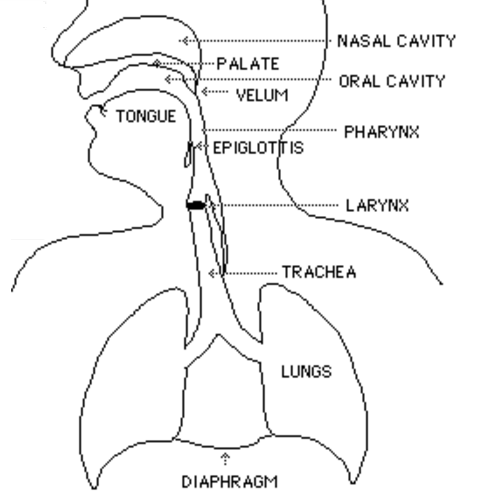
\includegraphics[width=10cm]{human}
  \caption{The human speech production system. Copied from \cite{vocal}.}
  \label{fig:human}
\end{figure}

\newpage
\textbf{Speech synthesis} is the artificial production of human speech using a computer, either hardware or software. A text-to-speech synthesis system is a system that converts written text to speech. There are two main steps in text-to-speech-synthesis. These are known as text analysis and speech waveform generation. In the text analysis phase, an input text is converted into phonetic or other linguistic format. In the second step an audio output is formed. Figure \vref{fig:tts} shows this operation. [2,2].

\begin{figure}[h]
  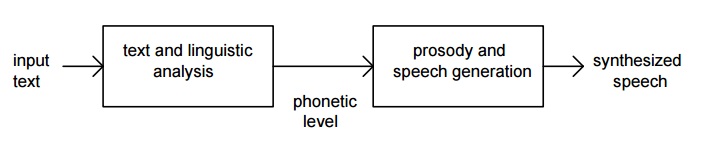
\includegraphics[width=15cm]{tts}
  \caption{Simple text-to-speech synthesis procedure. Copied from \cite{hut}.}
  \label{fig:tts}
\end{figure}

%Producing speech artificially is challenging partly because continuous speech is a set of complicated audio signals. Speech signals are divided as voiced and unvoiced. But sometimes something in between occurs. Voiced sound consist of fundamental frequency (F0) and its harmonic components. Each formant frequency also has an amplitude and bandwidth. 
%
%Fundamental and formant frequencies are usually the most important concepts in speech synthesis. With purely unvoiced sounds, there is no fundamental frequency in excitation and therefore no harmonic structure and the excitation can be considered as a white noise. When whispering a voiced sound there is no fundamental frequency in the excitation and the first formant frequencies produced by vocal tract are perceived. One way to represent speech signals is using time and frequency domain graph.  Figure \vref{fig:freq} shows speech signals of three vowels (/a/ /i/ /u/) presented as time and frequency domain. Fundamental frequency is about 100 Hz in all cases. \cite{hut}
%
%\begin{figure}[!h]
%  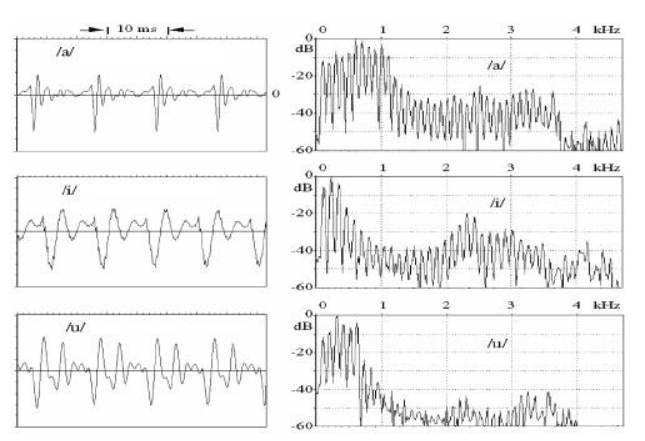
\includegraphics[width=12cm]{freq}
%  \caption{The time- and frequency-domain presentation of vowels /a/, /i/, and /u/. (Copied from \cite{hut}).}
%  \label{fig:freq}
%\end{figure}

The main objective of this theoretical background section is to examine the historical background, current status, architecture and design process of speech synthesizers. The materials for the literature review are mainly collected from on-line sources. Later the review will be used in an implementation of an existing speech synthesis system in developing an application targeted at assisting language learning.


\section{Brief history of speech synthesis}
%History
The first attempts to build artificial speech were carried out using mechanical devices to produce vowels. Later in the 1920s the first electrical synthesizer was introduced by Stewart. The synthesizer was capable of generating sounds of single static vowels. In 1939 VODER was introduced in the New York World fair. It was seen as the first speech sythesizer.  In 1953 the Parametric Artificial Talker (PAT) was introduced and it was considered as the first formant synthesizer. It had three formant resonators connected in parallel. The first integrated circuit speech synthesis system is perhaps the Votrax chip. In 1980, Texas Instruments introduced a product based on a low cost TMS-5100 chip called Speak-n-Spell which was designed to be a reading aid to children. Modern speech synthesis systems employ more sophisticated algorithms such as hidden Markov models (HMM) and neural networks. \cite[4-10.]{hut}

%applications, quality
Text-to-speech systems are now employed in a variety of applications including assistive tools, education, telecommunication, entertainment, navigation guidance, improving literacy \cite{rose2007plato} and as an alternative way for human-computer interaction (HCI). Clarity and naturalness are used to rate the quality of a speech synthesis system. \cite[79.]{hut}

\section{Speech synthesis techniques}
%methods
Currently one of the main methods used to create a speech synthesis system is by concatenating recorded speech units like phones or diphones.  Sometimes the speech units could even be words and sentences for specific usage domains. \cite{allen}. Another methodology commonly known as formant synthesis or rule-based synthesis uses an  additive synthesis and acoustic model. In a formant synthesizer the parameters of an input signal are varied to form  artificial speech. \cite{burk}. In addition to the above mentioned methods, Articulatory synthesis is a method that simulates human vocal tract and HMM-based synthesis implements Hidden Markov Model algorithms in speech synthesis \cite{hut}.

%\begin{figure}[h]
%  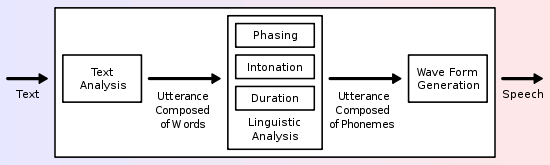
\includegraphics[width=15cm]{TTS_System}
%  \caption{Overview of a TTS system}
%  \label{fig:TTS_System}
%\end{figure}

%formant synthesis
The Source-filter-model of speech is used as a basis for formant synthesis. The formant-based synthesis technique is regarded more flexible because an infinite number of sounds could be produced. Intelligible speech requires at least three formants. Every formant is modeled with two pole resonators. This enables the formant frequency as well as bandwidth to be specified. A cascade formant synthesizer comprises band-pass resonators which are connected to one another in series \cite{hut} as shown in figure \vref{fig:cascade_formant_synthesizer}.

\begin{figure}[h]
  \centering
  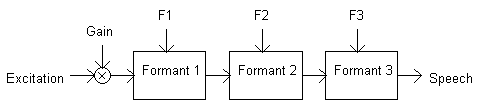
\includegraphics[width=15cm]{cascade_formant_synthesizer}
  \caption{Cascade formant synthesizer. Copied from \cite{hut}.}
  \label{fig:cascade_formant_synthesizer}
\end{figure}

%espeak

ESpeak is an open-source software implementation of a formant type synthesizer. It can use either its own espeak engine or Klatt. Voiced speech sounds such as vowels and sonorant consonants are created by adding together sine waves to make the formant peaks. Unvoiced consonants are made by playing recorded sounds. Voiced consonants are made by mixing a synthesized voice with a recorded unvoiced sound. Klatt uses the same formant data but produces voiced sounds by starting with a waveform and applying digital filters. \cite{espeak}

%development process: concatenative
The Unit selection method uses a large recorded speech data sufficient to cover a language features and then speech is produced by cutting and stitching units from a database\cite{chala}. Concatenation method depends mainly on runtime selection and compilation of speech units from database. For example, according to Acapela Group speech synthesis process for the word \textbf{impressive} is made up from chunks from the words "\emph{imp}ossible", "\emph{presi}dent" and "detect\emph{ive}" which results in a natural sounding word.
%comparison of the the systems
According to Silen et al., Speech synthesis based on unit selection can produce more natural sounding voice than other methods\cite[1]{silen} 
On the contrary to concatenative systems, formant based synthesis does not initially use a recorded human voice and as a result the output sound is more robot-sounding. However the main advantage of these systems is the smaller footprint of the programs due to lack of large database. Additionally the output voice does not suffer from glitches and a faster output could be produced.\cite{allen}


%case study finnish
A development of unit selection speech synthesizer developed for Finnish language in Tampere University of Technology illustrates the process of unit selection concatenative synthesizer. This method uses large pre-recorded speech inventory so that sufficient phonetic and prosodic coverage for a language is provided. As the name indicates units are cut and concatenated from a database to produce speech. Unit selection from database is guided by two costs, \emph{target} and \emph{join cost}.  The former measures similarity of candidate and desired units. On the other hand, the later measures the concatenation quality of two consecutive units. The design of database is important and should consider the target language because the quality of synthesized speech highly depends on coverage of the database.

To design a unit selection speech synthesizer, first and foremost understanding of target language is important even-though a unit selection synthesizer could be built with no or little knowledge of the target language\cite{silen}. Hence the authors, who developed unit selection Finnish speech synthesizer at TUT, studied the phoneme and orthography of the Finnish language and what makes it similar and different from other languages. Secondly a database was designed to store phonemes from a recorded speech units. Next, a synthesis engine was implemented and tested. 

A good example that implements diphone based synthesis is MBROLA project. A diphone is an adjacent pair of phones. Building new voices for MBROLA is efficient using diphone and sentence extraction tools. Diphone database is diphone synthesizer and it has to include all possible diphones in the language it is designed for. The general procedure of MBROLA voice creation is as follows:

The first step is \textbf{creating text corpus}. Here list of phones including allphones for a given language is prepared followed by a list of diphones. Then
a list of words containing all the diphones is created and each diphone should appear at least once. This is followed by putting a keywords in a career sentence. Next step is \textbf{recording the corpus}; The corpus is read by a professional speaker with monotonous intonation and  the speech is digitally recorded and stored in a digital format. After this the \textbf{corpus is segmented}. Here the diphones must be found and annotated and then position of the border between the phones is marked. Finally \textbf{leveling} is done. Here the energy levels at the beginning and end of a segment are averaged and pitch is normalized. After these steps diphone files are saved in a WAV format along with the diphone database file. \cite{jolanta}

\section{Computer assisted language learning (CALL)}
According to Philip Hubbard, Computer assisted language learning is defined as any process in which a learner uses a computer and as a result improves his or her language. It is a broad and dynamic field of study. Here, by computer it means in its broadest sense, including networks and other portable devices. By improving it means from various perspectives such as learning effectiveness, access to various learning materials, convenience across a wide range of time and place, motivational aspects and less or fewer expensive resource requirements.\cite{hubbard}

With regards to learning skills such as listening, speaking and pronunciation, computers and networks have evolved that large amount of information is readily available. These days listeners have access to a wealth of audio and video materials to listen from usually for free. In the future of language learning, the primary question will be how users choose materials that match their learning styles rather than which programs offer what kind of features. Speaking exercises could be accomplished via user taking to each other through an IT medium or users recording their sounds and playing it back. Automatic speech recognition systems could also be utilized. Pronunciation learning could be applied where by students trying to match their pronunciation relative to the one produced by a native speaker. Graphic representations of speech as a waveform, for example, could help for comparing the sounds produced by a student to a native speaker.\cite{hubbard}

Computer programs could assist reading and writing in multiple ways. In addition to the availability of multiple print materials in an accessible way, collaborative writing methods such as Google Docs have provided a way to write and share at the same time. Spelling, grammar and thesaurus checkers and on-line dictionaries also fit in the context of reading and writing with CALL.\cite{hubbard}

\section{Language learning and technology}
%how to reference informal materials???
Vast amount of materials is accessible on-line for various languages. Informal form of learning could take many kinds of approaches. As an example gaming and other fun ways of on-line collaboration is one form of an informal learning. Additionally, Peer to peer networks on various subjects, on-line dictionaries including translation services can be used by learners in developing their skills. For developing skills in vocabulary, there are programs like Quizlet and other flash card apps. Furthermore, for a longer term vocabulary retention, there exist advanced algorithms that help students to maintain optimal rhythm through time. Pod-casts and various video materials help in advancing listening comprehension. 

While the amount of information for an independent learner could be overwhelming, one can personalize his/her individual experience. There is a great potential in using personalized on-line resources. Mobile phones have brought high level of personalization in that they can be used in and out of class and information could be looked up with out restriction of place.

\section{Finnish phonetics and phonology}
While studying about speech technologies, it is important to know the characteristics of a target language. A phoneme is the smallest unit of speech that can be used to make one word different from another word. Phonemes are divided into consonants and vowels. In Finnish language there exist eight vowels. These are  /ɑ/, /e/, /i/, /o/, /u/, /y/, /æ/ and /ø/. Vowels can occur in both short and long form and sequences and diphthongs, which are adjacent vowel sounds occurring within the same syllable.\cite{silen} Figure\vref{fig:vowels} summarizes categorization of Finnish vowels.
Finnish orthography is phonemic: each phoneme corresponds to a certain grapheme (smallest unit in a writing system). One or more syllables exist in every word. Each syllable in Finnish has a vowel as a sonant, which means that every word has at least a vowel. 

\begin{figure}[h]
  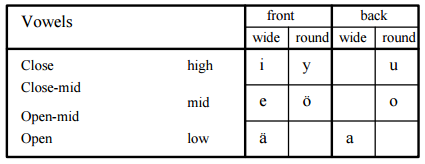
\includegraphics[width=12cm]{vowels}
  \caption{Classification of Finnish vowels. (Copied from \cite{hut}).}
  \label{fig:vowels}
\end{figure}

Depending upon the place of articulation consonants in Finnish are classified as plosives (vocal tract is closed causing stop), fricatives (vocal tract is tightened over some spot that the turbulent air creates sound), nasals (vocal tract is closed however velum opens a course to nasal cavity), tremulants (top of the tongue is vibrating), laternals (the top part of the tongue shuts the vocal tract) and semivowels (almost like vowel but unstable). Figure \vref{fig:consonants} summarizes Finnish consonants.\cite{hut}

\begin{figure}[h]
  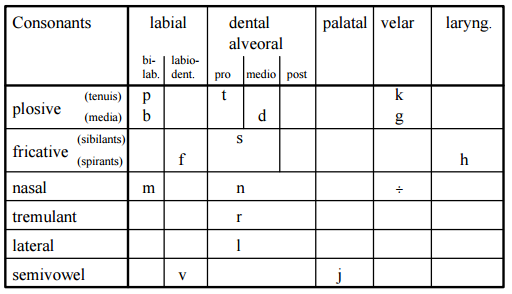
\includegraphics[width=14cm]{consonants}
  \caption{Classification of Finnish consonants. (Copied from \cite{hut}).}
  \label{fig:consonants}
\end{figure}

%\begin{figure}[h]
%  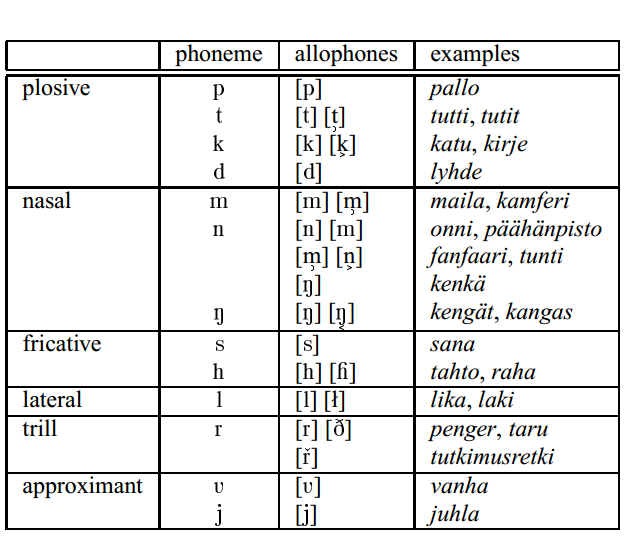
\includegraphics[width=12cm]{finnish}
%  \caption{Finnish consonants and their allophones (Copied from \cite{silen}).}
%  \label{fig:finnish}
%\end{figure}

\section{Natural language processing}

Natural language processing (NLP) is a field of computer science, artificial intelligence and computational linguistics concerned with the interactions between computers and human languages. Main challenges of the field include natural language understanding and natural language generation.

Natural language processing in the context of speech synthesis comprises of various elements. Figure \vref{fig:nlp} illustrates the role of natural language processing in a unit selection TTS system. As shown in the figure, when a given text is fed into parsing and structural analysis module, text boundaries are identified. These identified sentences are then fed to normalization module. Here numbers, addresses, acronyms and other special tokens are identified and expanded and converted to spoken forms.  Figure \vref{fig:rawtext} shows basic text processing. Text processing phase includes text to phoneme conversion, which is undertaken based on syllable to phoneme conversion rules.

\begin{figure}[h]
  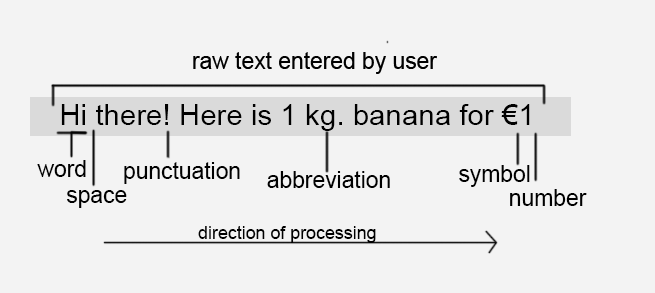
\includegraphics[width=12cm]{rawtext}
  \caption{Raw text processing.}
  \label{fig:rawtext}
\end{figure}
 The normalization module depends on lexicons and rule based approaches. Prosody module determines pitch contour, duration and intensity of the text to be synthesized. In general the NLP module is responsible for parsing, analyzing and transforming the input text to an intermediate symbolic format suitable to be processed using the DSP (Digital Signal Processing) module. \cite{chala}.

Natural language processing systems are widely used in commercial language applications. Apples Siri and Google now use these technologies. Deep neural networks implement large datasets and have great potential for use in language learning.

\begin{figure}[h]
  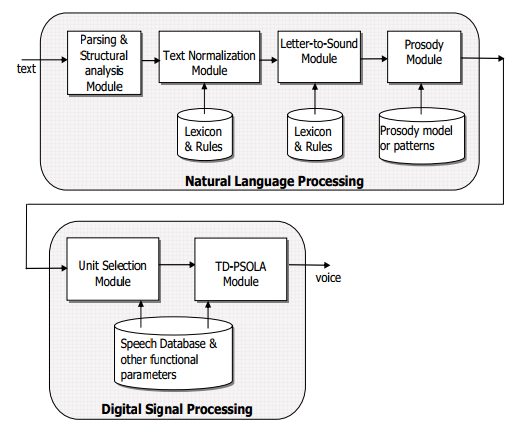
\includegraphics[width=12cm]{nlp}
  \caption{Architecture of unit selection TTS system (Copied from \cite{chala}).}
  \label{fig:nlp}
\end{figure}


\section{Applications of synthetic speech}
Many applications could benefit from the use of a synthetic speech. There have been products from talking toys and calculators to personal assistant applications in modern smart-phones that could conduct dialog with the user. In cases like warning and announcement systems, unrestricted vocabulary might not be required and simply recorded units of words and sentences could come to use. However for applications like reading applications for the blind, require a TTS system with unlimited vocabularies.\cite{hut}

Perhaps the most useful application of speech synthesis is to be used as communication aid for the blind. Before the common use speech synthesis, audio books used to be recorded by a professional speaker for use with the blind. This technique is expensive and time consuming. Nowadays, there exist applications that could be used to read aloud information from computer screen.

Synthetic speech can provide voice for people who are born-deaf and people who have difficulties in speaking. Subsequently it provides a chance to communicate with people who do not comprehend a sign language. Talking heads could improve the quality of communication since any visual type of information is very important for people who couldn't hear.

Other important area of application for synthetic speech is educational situation. For example language learning applications could make use of synthesized speech to teach pronunciation. It could be used to teach people who have impairment for reading (dyslexics).\cite{hut} Additionally synthetic speech could also be used together with spoken dialog systems in personal assistant applications, for proofreading with word processors, to read aloud email and SMS messages etc.


%\section{Conclusion}
%conclusion

\clearpage
\chapter{Available tools and techniques}

\section{Available speech synthesis products and APIs}
Many companies offer text to speech APIs to their customers in order to accelerate development of new applications utilizing TTS technology. These companies include AT\&T, IVONA, Neospeech, Readspeaker. In addition to these, major mobile operating systems like Android, IOS and Microsoft Windows offer API for text to speech. 

%Figure \vref{fig:finnish_resources} shows the availability of speech technology resources for the Finnish language. The figure is scaled from 0 to 5 and from the figure one can conclude that speech synthesis technologies are relatively well supported.

%\begin{figure}[h]
%
%  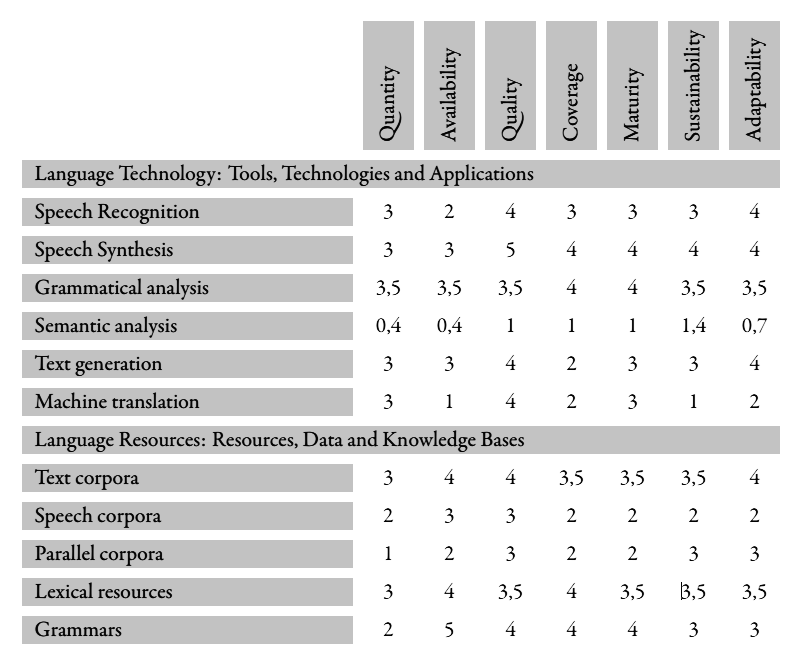
\includegraphics[width=12cm]{finnish_resources}
%  \caption{Availiability of  language technology resources for Finnish language (Copied from \cite{kopka}).}
%  \label{fig:finnish_resources}
%\end{figure}


%The following qualifications were used in the comparison of existing text to speech systems.
%\begin{itemize}
%  \item Support for languages
%  \item Voice quality (Natural sounding)
%  \item Ease of use
%  \item Voice control
%  \item Cost
%\end{itemize}

Available list of speech synthesis products was found using an on-line search. The following tools had been selected for testing, Listed in alphabetical order. Sample voices from these applications has been attached with this document on a CD. 

\textbf{Acapela}\\
Acapela Group is a company which develops text-to-speech software and services. It was formed from a combination of three companies that specialize in voice technology. Babel Technologies (Belgium), Infovox(Sweden) and Elan Speech (France). At the moment, Acapela has natural sounding voices for 25 languages including Finnish and has an API access for the cloud based TTS services. The service could be accessed though HTTP. Pricing is based on voice units.\cite{acapela}

\textbf{Espeak}\\
Espeak is a compact open-source speech synthesizer that supports many languages. It is available for Linux and Windows. Since it uses formant synthesis method, synthesized voice is not natural sounding. Espeak is available as a command line utility or as a dynamic library(DLL). It has also been ported to other systems like android and Mac OSX. \cite{espeak}\\

\textbf{Festival} \\
Festival is a framework for building speech synthesis systems and offers full TTS through a number of APIs. It is distributed with unrestricted license for commercial and non-commercial use alike. \cite{festival}

\textbf{Google}\\
Google text to speech system is primarily developed for Android operating system. It powers applications to read aloud the text on the screen. It has support for multiple languages. Google services like Google Translate use the system. The service provides API to developers in android platform. There also exist an unofficial access to the API by using the Google Translate service. Google TTS has been implemented in Chrome web browser to read any text in the browser. 

\textbf{Ispeech}\\
iSpeech is a TTS service from a California based company which develops speech solutions for various platforms. The cloud services are free to implement in mobile platforms while it costs a small fee for web platform. The service supports about 20 languages and the voice is of human like quality. The company provides an API for developers for testing. \cite{ispeech}

\textbf{Microsoft}\\
Microsoft Speech API (SAPI) is an API developed by Microsoft and allows to use speech recognition and speech synthesis within windows applications. The SDK is integrated into the windows OS itself. Microsoft Office and Microsoft speech server are among the applications that use SAPI. The Speech API is distributed freely and can be shipped with any Windows applications that use speech technology. The recent version of the API is SAPI 5.\cite{microsoft}

\textbf{Nuance}\\
Nuance is an American company that develops speech technology solutions. Its speech technology powers the Apple Siri personal assistant.  Nuance speech technologies are available for embedded, mobile and cloud platforms. More than forty languages are supported by the services. The on-line service for developers is accessed through HTTP REST interface. The developer API is available freely for evaluation purposes. \cite{nuance}

\textbf{ReadSpeaker}\\
Readspeaker is a suite of web-based applications that use TTS technology to enable speech in websites and mobile platforms. The application supports more than 35 languages. API for developers supports programming languages such as Java, Objective C, PHP, ASP and Flash. Free trial is available for evaluation. \cite{readspeaker}

From the above speech synthesis systems two of them; i.e. Festival and Espeak are open-source and freely available for any uses including commercial. The voice quality of these systems doesn't necessarily match to those available from commercial companies. However these systems allow their applications to be installed on own server without restriction. This implies that these could be deployed even without need to an internet connection. The two systems have been selected for further use in the implementation phase.\\



\begin{table}[h]

 \caption{Text to speech products}
    \begin{tabular}{ | l | l | }
    \hline
    \textbf{Product} & \textbf{Supported languages} \\ \hline
    Acapela & more than 25  \\ \hline
    Espeak &  many    \\ \hline
    Festival &  more than 5 \\ \hline
    Google &  many    \\ \hline
    Ispeech & over 20  \\ \hline
    Microsoft &  many   \\ \hline
    Nuance & over 40  \\ \hline
    ReadSpeaker & more than 35\\ \hline
    \end{tabular}

\end{table}

\section{Speech synthesis markup language}
Speech Synthesis Markup Language (SSML) is an XML based markup language for speech synthesis applications. To drive interactive telephony service, it is often embedded in a VoiceXML scripts. However it may also be used alone for example in audio book creation. For assisting generation of synthetic speech in web and other applications, SSML provides rich markup language.The essential role of the markup language is to provide authors of synthesizable content a standard way to control aspects of speech such as pronunciation, volume, pitch, rate etc.  across different synthesis-capable platforms.\cite{w3}
A text to speech system that supports SSML is responsible for rendering a document to spoken output and for using the information in the markup to render document as intended by the author. SSML document creation could be done by automatically, by a human author or both. SSML document processing is done in six steps. These are shown in Table 2.\\

\begin{table}[h]

 \caption{Steps in SSML document processing}
    \begin{tabular}{ | l | l | l | }
    \hline
    No. &Step &Description \\ \hline
    1 & XML Parse & extracting document tree from content \\ \hline
    2 & Structure analysis  & formatting the way document should be read  \\ \hline
    3 & Text normalization  & converting written to spoken form\\ \hline
    4 & Text to phoneme  &  words to the smallest unit of sound  \\ \hline
    5 & Prosody analysis  &   set of features of speech such as pitch and speaking rate\\ \hline
    6 & Waveform production  & audio waveform generation  \\ \hline
  
    \end{tabular}

\end{table}

%begin{itemize} 
%\item XML Parse: extract document tree from content
%\item Structure analysis: the way document should be read
%\item Text normalization: converting written to spoken form
%\item Text to phoneme: words to the smallest unit of sound 
%\item prosody analysis: set of features of speech such as pitch and speaking rate
%\item waveform production: audio waveform generation
%\end{itemize} 


%SSML has the following set of elements and attributes:
%\begin{itemize} 
%\item Document structure, text processing and pronunciation:\\
%"speak" root element, 
%"xml:lang" attribute, 
%"paragraph and "sentence", 
%"say as", 
%"phoneme"
%\item Prosody and style:\\
%"voice",
%"emphasis", 
%"break", 
%"prosody", 
%\item Other elements:\\
%"audio", 
%"mark"
%\end{itemize} 

The following listing shows sample SSML
\begin{lstlisting} [caption = Sample SSML syntax]
<speak xml:lang="en-US">
<paragraph>this is a test</paragraph>
<paragraph xml:lang="fi">tämä on testi</paragraph>
</speak>
\end{lstlisting}

\section{Speech quality and evaluation}
Intelligibility, naturalness and suitability can be used to evaluate the quality of a synthetic speech. In some applications like reading use for the blind, intelligibility at high rate of speed is more important. On the other hand in multimedia applications, naturalness and prosodic features are more important. Evaluation could be carried out at various levels such as phoneme, word or sentence level based on what kind of information is required.\cite{hut}

Text processing and linguistic realization are important in a text to speech system just like the acoustic properties. For a good result different kinds of techniques should be used. Evaluation is often made by a subjective listening test with a response set of syllables, words, sentences. Usually consonants are more problematic to synthesize than vowels. Hence most test material is targeted to test consonants. Specially nasalized consonants such as (/m/ /n/ /ng/ ) are usually those which result in problems. 
%There are also some objective methods of testing like Articulation Index (AI) or Speech Transmission Index (STI).These methods may be used when a synthesized speech is through some transmission channel but not suitable to measure speech quality in general.
When a test procedure is repeated for the same listening group, the test results may increase significantly. This is caused because after every listening session the testers get more familiarized with the synthesized speech and understand it better.  \cite{hut}

%On the other side concentration problems may decrease the results especially in segmental methods. Hence using native or pro listeners is important in listening tests.\cite{hut}
 
\clearpage
\chapter{Current research in speech technologies}
The future of speech technologies depends on the current research undertaken in the field and identifying the promising directions.
Since 1990s advancements in computer software and hardware along with a better understanding of speech has allowed speech technologies to be deployed in enterprises. At the same time developments in the field of linguistics have led use of computers in the use of developing listening and speaking skills and second language acquisition. Some major language learning applications these days are using these technologies and new standards are being developed in this area.\cite{rob}

\section{Visualization of speech}
There has been tools to provide graphical representation of speech in computers since the 1990s. These are intended so that users could compare their pronunciation along with a native speaker of a language. However a little guidance was left to the user on how to improve pronunciation. Most language learning systems follow similar model in that learners first listen to a native speaker and then asked to produce their own.

Waveform representation of speech is one way to provide feedback to the user. But in addition to this the feedback could also be audiovisual including representation of mouth parts. One of the issues in traditional approaches to visualization of speech is difficulty users may have in understanding or interpreting the feedback displays. Some speech software developers have experimented with game-like interfaces in which a user controls a game character based on his/her correct pronunciation. In some ways a computer based pronunciation practice is more efficient. These include, when there is a one to one access for students with computer, when users are allowed to proceed with their own pace and a computer program is customized to the need of the student.\cite{rob}\\

Figure \vref{fig:viz} shows a program known as "Tell me more". This program implements a speech recognition in order to provide a score based on how close the user pronunciatimailon is relative to a native speaker's recording. In the program visual feedback is provided using audio waveforms and shows mouth parts used in the speech visualization.

\begin{figure}[h]

  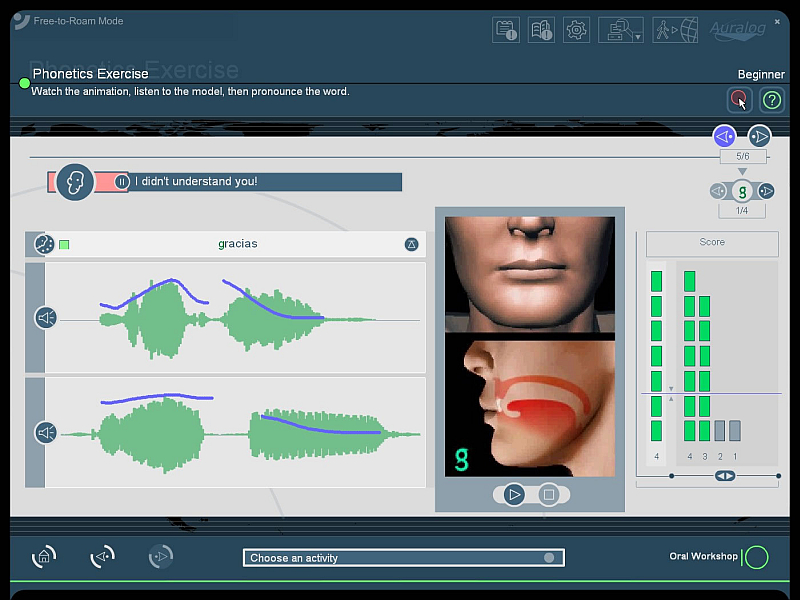
\includegraphics[width=12cm]{viz}
  \caption{Language learning application implementing visualization of speech (Copied from \cite{tellmemore}).}
  \label{fig:viz}
\end{figure}


\section{Automatic speech recognition (ASR)}
In the past decades, ASR has been an area of considerable interest in the signal processing and Human language technology (HLT) communities.\cite{baker} Despite the growing practical applications a significant development in ASR is expected in the future. It is expected to be world wide deployed. This could be expected due to the growth of technology in infrastructure, knowledge representation and increasingly advancing algorithms. Moore's law predicts that doubling amount of computations achievable for given cost in every 12 to 18 months as well as shrinking cost of memory. These developments has enabled researchers to run more complex algorithms in a short time. Increasing availability of speech corpora has led automated systems to achieve proficiency. For instance, various national institutions along with educational ones have provided research tools such as hidden Markov model toolkit (HTK), Sphinix etc.

%\begin{figure}[h]
%  \centering
%  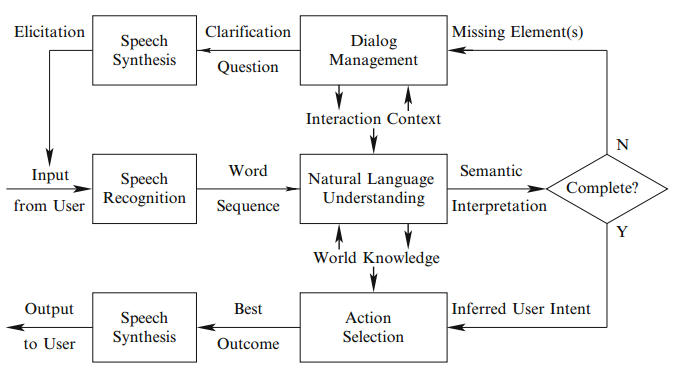
\includegraphics[width=15cm]{spokendialogue}
%  \caption{Personal assistant interaction: implementing speech synthesis and recognition (Copied from \cite{markowitz}).}
%  \label{fig:spokendialogue}
%\end{figure}

Audio indexing and mining have enabled high-performance automatic topic detection as well as applications for automatic speaker detection. Current ASR systems perform poorly when encountering audio signals that differ from the limited conditions under which they were developed.
This focused research area would concentrate on creating and developing systems that would be more robust against variability and shifts in acoustic environments, such as environmental noise and various speaker conditions.\\
The major change in speech analysis was the introduction of statistical methods like Hidden Markov Model (HMM), thirty years ago and still prevails. A number of new models have been introduced and expected in the future to come.
Rapid portability to emerging languages is the other domain. Todays top ASR systems are not readily available for all languages and hence the goal in the future is in the direction that spoken language technologies are easily portable.

\section{Standards}
Making of a software with speech technology has been difficult due to the fact that there has not been commonly accepted standards. However this has been changing recently because of efforts made by various sectors. W3C's (World Wide Web Consortium) effort to develop speech related standards can be a good example. Some interesting projects that use the web include SPICE from CMU whose main merit is to create an ASR for rare languages. These projects use the web and they are able to learn and improve through time. Increased use of multimedia such as videos together with speech technologies and incorporation of natural speech is becoming common. Virtual reality games have been increasingly using speech technologies and an increasing implementation of speech technologies in mobile technologies is expected to continue. Some of the institutions which are conducting research in speech technologies include the following.\\
\begin{table}[h]
 \caption{Some institutions conducting research in speech technologies}
    \begin{tabular}{ | l | l | }
    \hline
    \textbf{Institution} & \textbf{URL} \\ \hline
    IBM research, & http://www.research.ibm.com/tts/ \\ \hline
    Cambridge &  http://mi.eng.cam.ac.uk/research/dialogue/   \\ \hline
    Microsoft research &  http://research.microsoft.com/en-us/projects/whistler \\ \hline
    John Hopkin university &  http://www.clsp.jhu.edu/   \\ \hline
    AT\&T Natural Voices & http://www2.research.att.com/~ttsweb/'/demo.php\#top  \\ \hline
    \end{tabular}
\end{table}

\section{Emerging markets in mobile speech}
There is a growing diverse market for mobile speech technologies. Mainly these new markets include Warehouse operations, offender monitoring and robotics. With the emergence of Siri, recent focus has been on personal assistants for smart phones. This has led the creation of competitors to Siri such as Nina (Nuance communication), Lola (SRI international), Lexee (Angel labs) and Watson for smart phones(IBM). \cite{markowitz}

"Eyes busy", "hands busy" environments in factories and warehouses were among the earliest markets for mobile speech. These include manufacturing inspection, sorting, order picking, return processing etc. A workers eyes and hands need to be focused on the tasks to safely perform the tasks so that errors and accidents do not occur. \\ Starting from the 1980s these eyes-busy tasks were well suited to speech technologies. The alternatives like pausing tasks to write findings on data-sheet is error prone or even using additional data-clerks to write using for example a laptop is costly. Since factory users do repetitive tasks every day the vocabularies for speech technologies could be limited and users could train their own voices. For example figure \vref{fig:orderpicking} provides an example of spoken dialog interaction of a factory worker with a system. In these factory environments the main challenge has been noise. For this, speech technology companies have for example used noise canceling microphones and sometimes embedded the mic into hard-hats or protective ear-ware.\cite{markowitz}

\begin{figure}[h]
  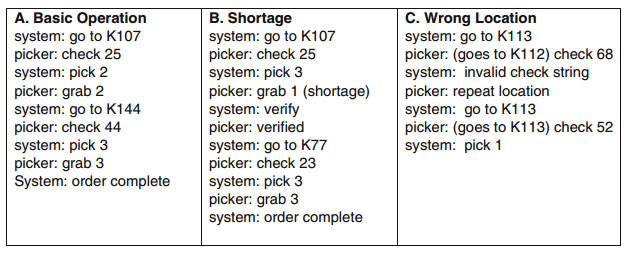
\includegraphics[width=15cm]{orderpicking}
  \caption{Order picking. Example drived from demo video produced by Voxware (copied from \cite{markowitz})}
  \label{fig:orderpicking}
\end{figure}



Correction facilities ware among the largest market for speaker verification. The main reason for using this technology is the increase in alternative sentencing for non violent offenders. Heavy caseloads made it increasingly difficult for officers to monitor offenders effectively.\cite{markowitz}

Despite the extreme capabilities of robots in speech in various science fiction, there exist few actual robots that utilize speech. There exist two categories: robots which are able to respond to pre-defined speech and those who can learn and use language (autonomous robots). There exist toys which can accept commands via voice and respond either in action or using speech synthesis. Additionally there are worker robots developed for special needs people. For example hospital bed controlled by voice. \cite{markowitz}

\clearpage
\chapter{Implementation}

Many speech technology companies provide TTS solutions. From these there exist a number of natural sounding Finnish text to speech systems. Designing a new text to speech system from scratch is beyond the scope of this thesis. However some existing text to speech systems will be used in an experement to build a web based application  intended in assisting language learning. The main features of this application will be synthesizing user text into speech and using speech recognition for pronunciation practice. Text to speech engines will be installed on a server and the client side app communicates with the server using HTTP GET method. Overall the implementation plan is such that a user entered text is sent to the server first. Then after a speech is synthesized on the server the resulting audio is sent back to the client side.  Figure \vref{fig:clientserver} illustrates the client and server architecture.

\begin{figure}[h]
  
\includegraphics[width=12cm]{clientserver}
  \caption{Client and server architecture}
  \label{fig:clientserver}
\end{figure}


\section{Setting up a Linux text to speech server }
In order to have a web interface to the speech engines installed, a server environment is set up. The server for this demo was Ubuntu 14.04 LTS and it was installed as a guest system into a virtual machine. A complete LAMP (Linux Apache MySQL and PHP) stack was installed in the server environment. On the server side PHP script accepts user text from browser and returns synthesized audio. On the other hand Jquery and Javascript were used for the client side web application. 

Espeak and Festival text to speech systems were selected for the experement. Espeak supports various languages including Finnish. It can be easily installed to a Linux system from Linux repositories. Similarly Festival is found in the Ubuntu  package repositories. However Finnish voices for festival are not pre-installed along with festival and have to be downloaded separately. Finnish Festival voices have been developed in the University of Helsinki as part of Suopuhe project and are available in Ubuntu and Debian repositories. 


\subsection{Espeak}

Espeak is an open source software and is available for Linux, Windows and MacOSX operating systems. Additionally there exists an Espeak port to the android platform. 

Espeak is a formant type rule based speech synthesizer. A text to be synthesized is first converted into phoneme. Phoneme is the smallest linguistic unit. There exist different set of phonemes for different languages. For example English has 41 phonemes as defined by International Phonetic Association (IPA). Espeak uses some rules to convert a text to the phonemes and allophones (variation of phoneme). Hence the program has smaller memory consumption when compared with dictionary based speech synthesis systems.


Below is a list of some command-line parameters of Espeak. For a simple text synthesis the following is used\\
\textbf{espeak} "this is a test" or \textbf{espeak} -f <text file>\\
%or\\
%\textbf{espeak} followed by return then writing text and pressing enter\\
The basic syntax is as follows\\
\textbf{espeak [options] ["text words"]}\\
Some basic options for synthesis include:\\
\textbf{-w <wave file>}\\
writes the speech output to a file in a WAV format instead of speaking it aloud.\\ 
\textbf{-v <voice filename>[+<variant>]}\\
sets voice for the speech, usually to select a language. For example the following command sets a Finnish voice.\\
\textbf{espeak} -vfi\\
In addition to these female and male voices are synthesized using variable pitch. These include +m1 +m2 . . . +m7 for male voices and +f1 . . . +f4 for female voices.

Additionally Espeak has parameters to control the synthesized voice's speed, pitch and amplitude.

Espeak allows users to add or improve additional languages. This consists of defining phoneme table for a language, spelling to phoneme translation rules and adding a file for pronunciation of symbols, numbers and abbreviations. Espeakedit is a program used prepare phonemedata and compile voices for espeak. A screenshot of espeakedit is shown in figure \vref{fig:espeakedit}

\begin{figure}[h]
  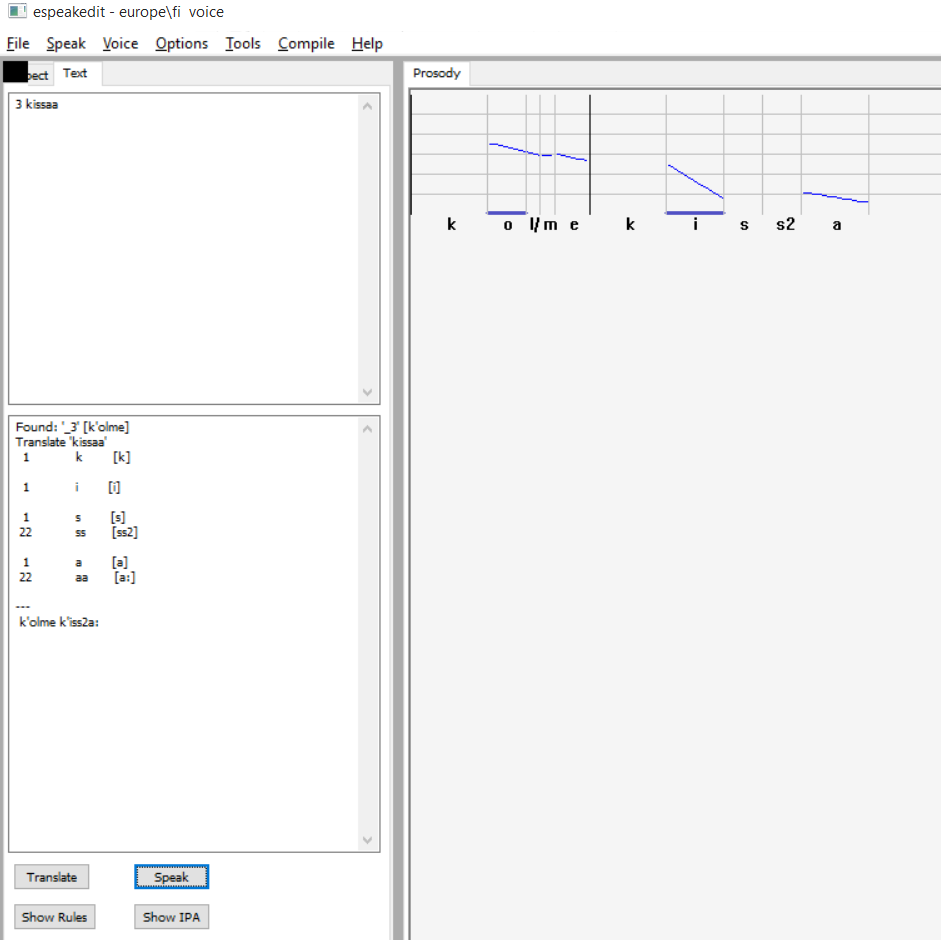
\includegraphics[width=15cm]{espeakedit}
  \caption{Espeakedit window}
  \label{fig:espeakedit}
\end{figure}

\subsection{Festival}
Festival is a multilingual text to speech system developed originally by Alan W. Black at University of Edinburgh. Festival works in two modes. Command mode and text-to-speech mode. When in command mode input (from file or interactively ) is interpreted by the command interpreter. When in text-to-speech mode, input is treated as text to be rendered as speech.
Festival's basic calling method is like:\\
\textbf{festival [options] file1 file2 ....}\\
In command driven mode festival is started with no arguments.
some useful command line options of festival are the following:\\
\textbf{--tts}\\
synthesize text in files as speech, if no file is given from standard input (stdin)\\
\textbf{--language} <string>\\
Run in named language

After eSpeak and Festival have been installed on the server, a small demo web application that uses these two engines is implemented. 



\subsection{Server side scripts}
On the server side PHP scripts are used to call the command line parameters of Espeak and Festival. These scripts accept a text as a GET parameter and pass it to either Espeak or Festival command line applications. Then the scripts return an audio from the synthesized voice in MP3 format. Sample server side code is shown in the listing below. Note here that \textbf{text2wave} comes along with festival installation and converts text to an audio in WAV format.

\lstset{language=php}
\begin{minipage}{\linewidth}
\begin{lstlisting} [caption =PHP script to use commandline festival]
<?php
$base_dir = '/tmp/';
$text = $_GET['text'];
$filename = md5($text) . '.mp3';
$filepath = $base_dir . $filename;
$text = escapeshellarg($text);
if (!file_exists($filepath)) {
  $cmd = "echo $text| iconv -f UTF-8 -t ISO8859-1 | text2wave |\
  lame --preset voice -q 9 --vbr-new - $filepath";
  exec($cmd);
}
header('Content-Type: audio/mpeg');
header('Content-Length: ' . filesize($filepath));
readfile($filepath);
?>
\end{lstlisting}
\end{minipage}
\section{Developing demo web application}
The client side application has three main pages. The menu page has links to these pages. These are "Read Stories" and "Listen Dialogue" and "Practice pronunciation". The initial menu page is shown in Figure  \vref{fig:menu}.
\begin{figure}[h]
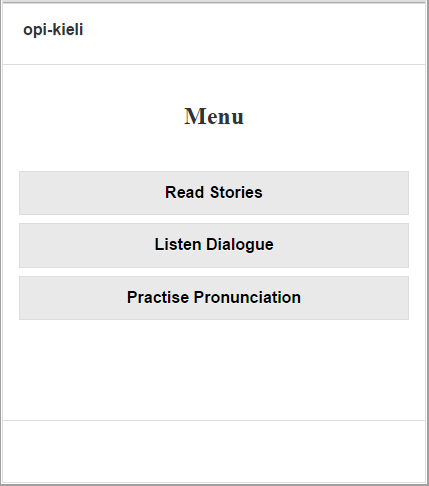
\includegraphics[width=7cm]{menu}
\caption{Applications menu page}
\label{fig:menu}
\end{figure}

Read stories page is a place where user can hear to stories read aloud by text to speech engines. On this page a user could input his/her own text to the blank space and then listen a story. Sample text could also be fetched by the user for testing. Figure  \vref{fig:reading} shows the Read stories page.

\begin{figure}[!ht]
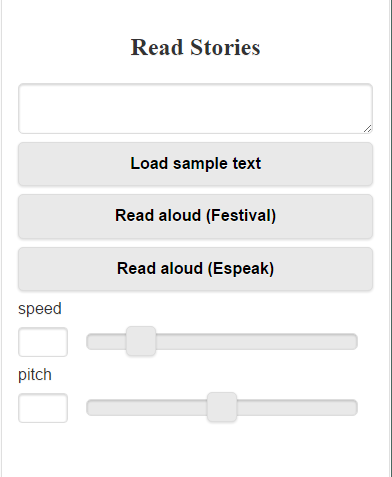
\includegraphics[width=7cm]{reading}
\caption{ Read Stories page}
\label{fig:reading}
\end{figure}

The load stories page leads to a list of stories. These stories are saved as text files on the server and loaded with using Ajax synchronously. \\ Below is a function that loads text file into a browser.


\begin{minipage}{\linewidth}
\begin{lstlisting} [caption =Function that text file synchronously using ajax]
function loadfile(filename) {
    /*
    Function: loadfile
    loads file given on the parameter using ajax synchronous
    Parameters:
    filename - the file name to be loaded                            
    See Also:       
    */
    $.ajax({
        async : false,
        url : filename,
        success : function(data) {
            story1 = data;
        }
    });
}

\end{lstlisting}
\end{minipage}

On the client side the following javascript function sends text to be synthesized and plays the resulting audio obtained from the server.

\begin{minipage}{\linewidth}
\begin{lstlisting} [caption =Function that sends text to server]
function speak(text) {
    /*
    Function: speak
    speaks aloud using an on-line speech service.
    See Also:						
    */
    var audio_src = "http://ttss.com/f.php?text='"+text+"'";							
    var audio = document.getElementById('speakaudio');
    audio.src = audio_src;
    audio.play();						
}
\end{lstlisting}
\end{minipage}



The Listen Dialogs has conversational phrases between two speakers. A set of dialogs is shown on a given page. User clicks on the dialogs to hear it aloud. A sample dialogs page is shown in figure \vref{fig:dialogue}.

\begin{figure}[h]
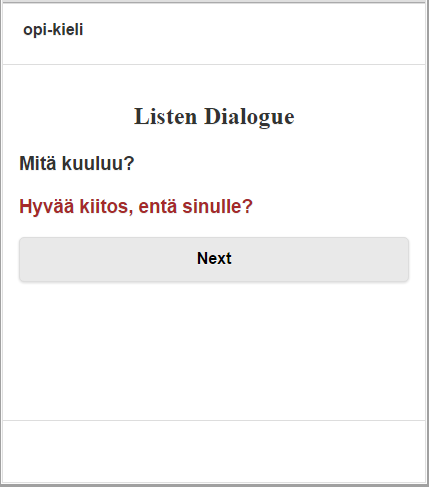
\includegraphics[width=7cm]{dialogue}
\caption{Listen Dialogue page}
\label{fig:dialogue}
\end{figure}

%Finally the Practice Pronunciation page provides sample phrases with a graphical waveform as spoken using text to speech engine. Users press the record button  and practice the words/phrases loudly. Users will be able to compare the waveform images of their pronunciation along with the speech engine. For this page it has been assumed that the speech engines pronunciation is closer to a native speaker than to a learner. Pronunciation page is shown in figure \vref{fig:pronunciation}.
The practice pronunciation page features speech recognition that uses Google's technology as a back end. On this page a user could try a word with a speech synthesizer and at the same time practice pronunciation using a microphone as an input.
\begin{figure}[h]
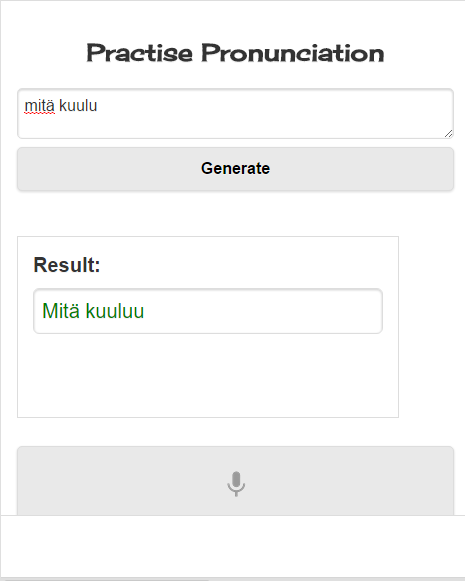
\includegraphics[width=7cm]{pronunciation}
\caption{Practice Pronunciation page}
\label{fig:pronunciation}
\end{figure}

On the client side, Jquery mobile was used to design the demo web application. Jquery mobile allows creation of responsive web based mobile applications.

%Generating waveforms from synthesized voice is done using a tool called Sox. Sox is a commanline utility for sound manipulation. To generate a visual from %the audio files being synthesized:
%\begin{verbatim}
%sox "audio_file.mp3" -n spectrogram -Y 130 -l -r -o "image_file.png"
%\end{verbatim}

Generating a waveform image from a user's audio input was one of the initial ideas in the project. Python based script was used to generate a waveform from audio recording. Here a user could produce visuals from synthesized audio to compare it with his own speech. Despite the fact that this solution was not integrated into the project, it was found important during development for demo purposes. Figure \vref{fig:python} shows a script that generates audio waveform  from an audio input.

\begin{figure}
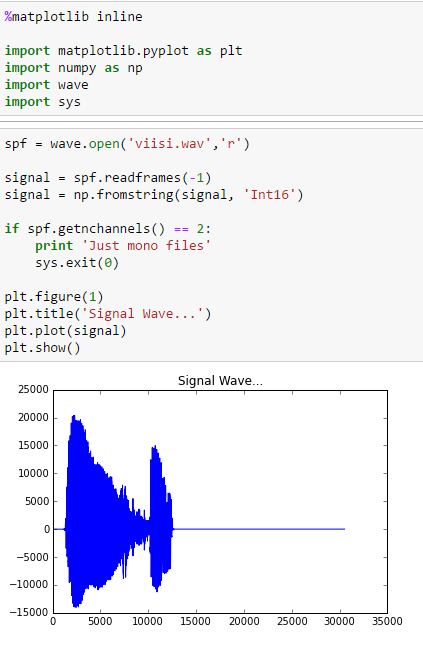
\includegraphics[width=11cm]{python}
\caption{Python script to generate audio waveform}
\label{fig:python}
\end{figure}

%\subsection{Loading sample text}
%\subsection{Application Setup and Creating Database}
%\subsection{View Functions and Templates}
%\subsection{Adding Style}


\section{What was achieved }
At the moment speech technologies are developing in a fast pace, specially in the mobile market. In this project historical background, available techniques, current research and application areas of speech synthesis technology have been investigated.

There are quite many speech synthesis engines available on the market. Some products have been selected and compared. Then  two of them have been selected for further experiment. The main reason in the selection has been ease of availability for off-line use, being free of cost and open source. 

Speech technologies have an important role in language learning. A small web application has been developed in order to demonstrate the application of speech synthesis for education. Hence in summary two text to speech applications, Espeak and Festival have been selected for use in a small web application intended in assisting language learning.

\clearpage
\chapter{Conclusions}
At the moment there exist many speech technology companies offering products for the market. Additionally there is a lot of research in companies and educational institutes in the field. As a result the quality of speech synthesis systems has improved a lot that many systems could produce natural sounding and very intelligible voice. Some companies have even produced TTS solutions with children's voice. However some issues still exist like producing the right emotions in the synthesized speech. On the other hand several new applications that incorporate speech technologies have been developed. Apple's SIRI and Google Now have brought speech technologies for the mass and this has gained popularity as an alternative interaction method with mobile devices. Other new emerging markets in the industry include offender monitoring, robotics and warehouse operations.

Basic methods of speech synthesis have been covered in chapter two. These include formant based, concatenative and articulatory synthesis. Concatenative method has gained more popularity because more natural sounding output could be produced. On the other hand formant based synthesis is known for its smaller memory footprint and flexibility. Hence it has been popular in embedded technologies. Articulatory synthesis technology is still in research phase due to its complexity.

In this project a demo web application has been developed to illustrate the use of speech technologies in language education. This demo features two text to speech applications; Espeak and Festival. A user is able to use the application to read text aloud. It has been found that TTS technologies are important in such applications designed to assist language education.

There exist many natural sounding text to speech technologies for many of the European languages. However speech technologies are not equally available in every language. Some experiments were carried out to use Oromo language, one of the languages in Ethiopia, to read a text using a Finnish speech synthesis technology. From the experiments the output sound was close enough to good. This may have been due to similar features in vowel length and consonant gemination between the languages. 

Many of modern speech technology products are complex that it is difficult task to port them among languages. This is specially true when the speech technology is based on a recording, such as unit selection speech synthesis system. Hence portability of speech technologies among languages remains a work for the future. 

%Despite the fact that the application is not totally complete, a working demo has been developed and implemented.  There were problems with the 'practice pronunciation' section of the application. First, waveform is generated from synthesized voice instead of a native speakers recording, Second, there were technical problems while recording audio using a browser hence, the user had to record using the client side device's recording tool. This section has been revised so that the user uses a speech recognition service from google. To generate realtime waveforms from a user speech will be a task that remains for future development.
%
%In this short literature review the history, application areas and common methods used for a speech synthesis have been reviewed from different sources. Main techniques in use include concatenation and format based synthesis. The application areas have been growing and is being used in assistive technologies, education, telecommunication and multimedia among others. In the future speech synthesis has a promising future for being a better alternative human computer interaction mechanism.
\clearpage

%\section{Section}
%Here is an example how to add biblio entry \cite{allen:book} using the \textquotedblleft cite\textquotedblright ~\cite[section 4.2]{allen:book}. Note that a paragraph is added by forcing a new line.
%
%And let also try the figure (see figure \vref{fig:latex-cover}) and internal reference (with label and ref or vref). The reference can be done to any label, for example why not to appendix \ref{appx:first} or to appendix \ref{appx:second}? To note, \LaTeX{} will place the figure to the best place (except with forcing). Let them float till the final of final edit\ldots ~then force them to not break a paragraph.%hugly hack... I'm sorry
%\begin{figure}[h]
%  \centering
%  
\includegraphics[width=7.1cm]{LaTeX_cover}
%  \caption{\LaTeX{} cover image (Copied from wikibooks.org (2012) \cite{wikibooks:latex}).}
%  \label{fig:latex-cover}
%\end{figure}
%
%Let's also try a long quote:
%From the Universal Declaration of Human Rights:
%\begin{quote}
%(1) Everyone has the right to education. Education shall be free, at least in the elementary and fundamental stages. Elementary education shall be compulsory. Technical and professional education shall be made generally available and higher education shall be equally accessible to all on the basis of merit.
%
%(2) Education shall be directed to the full development of the human personality and to the strengthening of respect for human rights and fundamental freedoms. It shall promote understanding, tolerance and friendship among all nations, racial or religious groups, and shall further the activities of the United Nations for the maintenance of peace.
%
%(3) Parents have a prior right to choose the kind of education that shall be given to their children. \cite[article 26]{un:udhr}
%\end{quote}
%
%\textit{Quisque augue} est, \textbf{elementum ac porttitor} non, porttitor ac orci. Donec hendrerit, ligula ac luctus egestas, sem dolor pretium nunc, sed vehicula magna diam a massa. Donec mattis, arcu et tempor mattis, risus tortor ultrices metus, nec sodales sem dolor eu elit.\vspace{-17pt} 
%\begin{itemize}
%\item \textbf{A small hack} with list
%\item is to force the vertical space 
%\item before and after the list
%\end{itemize}
%\vspace{-17pt} Nullam egestas enim at odio pellentesque bibendum. 
%
%\subsection{Subsection}
%Donec et sapien ac leo condimentum vulputate id et tellus. Maecenas hendrerit malesuada interdum. Aenean dignissim sem faucibus elit congue faucibus id non risus. Morbi at dui non tortor pellentesque consequat non eget urna. Cras in sapien dui, a tincidunt velit.
%\reaction{\label{eq:reaktio}$\underset{\text{+II}}{\ce{2Fe^2+}}$ + $\underset{\text{+I\;-I}}{\ce{H2O2}}$ + $\underset{\text{+I\;-II}}{\ce{2H3O^+}}$ <=> $\underset{\text{+III}}{\ce{2Fe^3+}}$ + $\underset{\text{+I\;-II}}{\ce{4H2O}}$}
%Työn aluksi rauta(II)ionit hapetetaan rauta(III)ioneiksi väkevällä vetyperoksidilla, kuten reaktion~\ref{eq:reaktio} hapetusluvuista nähdään (rauta hapettuu, happi pelkistyy).  
%\reaction{Fe^3+( \emph{aq} ) + 3OH^-( \emph{aq} ) + $(x-1)$H2O( \emph{l} ) -> FeOOH $\cdot$ $x$(H2O)( \emph{s} )}
%Rauta(III)ionit saostetaan emäksen (\ce{NH3}) avulla ja saadaan tuotteeksi kidevedellinen rauta(III)hydroksidi. Saatu saostuma pestään \ce{NH4NO3}:lla.
%\reaction{FeOOH $\cdot$ $x$(H2O)( \emph{s} ) ->T[$\Delta$900-1000\celsius] Fe2O3( \emph{s} )}
%
%\subsection{Subsection with Math}
%Donec et sapien ac leo condimentum vulputate id et tellus. Maecenas hendrerit malesuada interdum. Aenean dignissim sem faucibus elit congue faucibus id non risus. Morbi at dui non tortor pellentesque consequat non eget urna. Cras in sapien dui, a tincidunt velit. Tertiäärinen butyylikloridi reagoi veden kanssa oheisen reaktion mukaisesti:
%\reaction{(CH3)3CCl + 2H2O -> (CH3)3COH+H3O+ +Cl-}
%Kyseessä on ensimmäisen kertaluvun reaktio, joten reaktion nopeus on
%\begin{align}
%v=-\frac{\mathrm{d}[\tn{t-ButCl}]}{\mathrm{d}t}=\frac{\mathrm{d}[\tn{HCl}]}{\mathrm{d}t}=k[\tn{t-ButCl}]
%\end{align}
%Jos tarkastellaan lähtöaineen t-butyylikloridin häviämistä saadaan
%\begin{align}
%\frac{\mathrm{d}[\tn{t-ButCl}]}{[\tn{t-ButCl}]}&=-k\mathrm{d}t \\
%\int \frac{\mathrm{d}[\tn{t-ButCl}]}{[\tn{t-ButCl}]}&=-k \int \mathrm{d}t \\
%\ln \int_{[\tn{t-ButCl}]_0}^{[\tn{t-ButCl}]} [\tn{t-ButCl}]&=-k\int_0^t t \\
%\ln \left( \frac{[\tn{t-ButCl}]}{[\tn{t-ButCl}]_0} \right)&=-kt
%\end{align}
%Ionivahvuus lasketaan kaavalla.
%\begin{align}
%I&=\frac{1}{2}\cdot\sum z_i^2c_i \\
%z_i&= \tn{ionin varausluku} \\
%c_i&= \tn{ionin konsentraatio}
%\end{align}
%Aktiivisuuskerroin $\gamma_\pm$ lasketaan kaavalla.
%\begin{align}
%\log \gamma_\pm &= -\left|z_+\cdot z_-\right|A\cdot I^{\frac{1}{2}} \\
%A &= \tn{0,509 (lämpötilassa 25\celsius}) \\
%I &= \tn{ionivahvuus} \\
%z &= \tn{ionien varaus}
%\end{align}
%
%\section{Section with Source Code}
%Donec et sapien ac leo condimentum vulputate id et tellus. Maecenas hendrerit malesuada interdum. Aenean dignissim sem faucibus elit congue faucibus id non risus. Morbi at dui non tortor pellentesque consequat non eget urna. Cras in sapien dui, a tincidunt velit.
%
%\vspace{-22pt}\begin{lstlisting}[language=PHP,caption={Descriptive Caption Text},label=testphp] 
%
%<?php
%$userName = $_POST["usern"];
%//maybe not?
%if ($userName){
%	?>
%	<h2>Hello <?php echo $userName; ?>!</h2>
%	<p>your message got received.</p>
%	<?php
%}
%?>
%\end{lstlisting}\vspace{-22pt}
%
%
%As see in listing \ref{testphp}: Donec et sapien ac leo condimentum vulputate id et tellus. Maecenas hendrerit malesuada interdum. Aenean dignissim sem faucibus elit congue faucibus id non risus. Morbi at dui non tortor pellentesque consequat non eget urna. Cras in sapien dui, a tincidunt velit.
%
%\section{Section with Table}
%Donec et sapien ac leo condimentum vulputate id et tellus. Maecenas hendrerit malesuada interdum. Aenean dignissim sem faucibus elit congue faucibus id non risus. Morbi at dui non tortor pellentesque consequat non eget urna. Cras in sapien dui, a tincidunt velit.
%
%\begin{table}[h]
%  \centering
%  \caption{Some data}
%  %IMPORTANT the caption must be before the tabular, so it will be on top of the table (there are other tricks to force it on top; but this one is straitforward).
%  \begin{tabular}{| l | >{\centering\arraybackslash}p{.5\textwidth} |}
%    \hline
%    Test 1 & test 1234 test \\
%    \hline
%    Some more date comes here & with more values and if the text is very long it will disappear out of the box unless you force the column size :( \\
%    \hline
%  \end{tabular}
%  \label{table:some_data}
%\end{table}
%
%
%As presented in table \ref{table:some_data}: Donec et sapien ac leo condimentum vulputate id et tellus. Maecenas hendrerit malesuada interdum. Aenean dignissim sem faucibus elit congue faucibus id non risus. Morbi at dui non tortor pellentesque consequat non eget urna. Cras in sapien dui, a tincidunt velit.
%
%\begin{table}[h]
%  \centering
%  \caption{Another table with tabularx}
%  \begin{tabularx}{.95\textwidth}{| l | >{\centering\arraybackslash} X |}
%    \hline
%    Test 1 & test 1234 test \\
%    \hline
%    Some more date comes here & with more values and if the text is very long it will disappear out of the box unless you force the table size :( \\
%    \hline
%  \end{tabularx}
%  \label{table:some_data2}
%\end{table}
%
%As presented in table \ref{table:some_data2}: Donec et sapien ac leo condimentum vulputate id et tellus. Maecenas hendrerit malesuada interdum. Aenean dignissim sem faucibus elit congue faucibus id non risus. Morbi at dui non tortor pellentesque consequat non eget urna. Cras in sapien dui, a tincidunt velit.
%
%\begin{table}[htbp]
%  \centering
%  \caption{Booktabs example}
%    \begin{tabular}{rrrr}
%    \toprule
%    t (s) & [HCl] & [t-ButCl] & $\ln\frac{[t-ButCl]}{[t-ButCl]_0}$ \\
%    \midrule
%    0     & 4,02  & 160,88 & 0,00 \\
%    10    & 63    & 101,9 & -0,46 \\
%    20    & 115,2 & 49,7  & -1,17 \\
%    30    & 141,3 & 23,6  & -1,92 \\
%    40    & 157,9 & 7     & -3,13 \\
%    50    & 161   & 3,9   & -3,72 \\
%    60    & 164,3 & 0,6   & -5,59 \\
%    70    & 163,5 & 1,4   & -4,74 \\
%    80    & 163,8 & 1,1   & -4,99 \\
%    90    & 164,1 & 0,8   & -5,30 \\
%    100   & 164,3 & 0,6   & -5,59 \\
%    \bottomrule
%    \end{tabular}
%  \label{tab:thisislabel}
%\end{table}
%
%\chapter{Second Chapter}
%
%Lorem ipsum dolor sit amet, consectetur adipiscing elit. Aliquam aliquam aliquam purus, in ornare nulla imperdiet molestie. Nam tempus erat eu dui rhoncus et vestibulum mi elementum. Ut porttitor elit sit amet justo dignissim sit amet sagittis massa egestas. Mauris sed dolor eget dui fermentum sodales ut eu nibh. 
%
%Quisque augue est, elementum ac porttitor non, porttitor ac orci. Donec hendrerit, ligula ac luctus egestas, sem dolor pretium nunc, sed vehicula magna diam a massa. Donec mattis, arcu et tempor mattis, risus tortor ultrices metus, nec sodales sem dolor eu elit. Nullam egestas enim at odio pellentesque bibendum. 
%
%Donec et sapien ac leo condimentum vulputate id et tellus. Maecenas hendrerit malesuada interdum. Aenean dignissim sem faucibus elit congue faucibus id non risus. Morbi at dui non tortor pellentesque consequat non eget urna. Cras in sapien dui, a tincidunt velit.
%
%\chapter{Third Chapter}
%
%Lorem ipsum dolor sit amet, consectetur adipiscing elit. Aliquam aliquam aliquam purus, in ornare nulla imperdiet molestie. Nam tempus erat eu dui rhoncus et vestibulum mi elementum. Ut porttitor elit sit amet justo dignissim sit amet sagittis massa egestas. Mauris sed dolor eget dui fermentum sodales ut eu nibh.
%\begin{figure}[htbp]
%  \centering
%    \begin{tikzpicture}
%        \pgfplotsset{width=12cm,
%        compat=1.3,
%        legend style={font=\footnotesize}}
%    \begin{axis}[
%    xlabel={c (mg/l)},
%    ylabel={A},
%    legend pos=north west,
%    ymajorgrids=true,
%    grid style=dashed
%]
%
%\addplot [only marks, blue] table {data.dat};
%\addplot [no markers, thick, red] table[
%x=c,
%y={create col/linear regression}] {data.dat};
%\addlegendentry{data}
%\addlegendentry{%
%$\pgfmathprintnumber{\pgfplotstableregressiona}x
%\pgfmathprintnumber[print sign]{\pgfplotstableregressionb}$}
%\end{axis}
%\end{tikzpicture}
%\label{fig:stdplot}
%\caption{Simple linear regression plot (cannot get $r^2$ value)}
%\end{figure}
%Quisque augue est, elementum ac porttitor non, porttitor ac orci. Donec hendrerit, ligula ac luctus egestas, sem dolor pretium nunc, sed vehicula magna diam a massa. Donec mattis, arcu et tempor mattis, risus tortor ultrices metus, nec sodales sem dolor eu elit. Nullam egestas enim at odio pellentesque bibendum. 
%
%Donec et sapien ac leo condimentum vulputate id et tellus. Maecenas hendrerit malesuada interdum. Aenean dignissim sem faucibus elit congue faucibus id non risus. Morbi at dui non tortor pellentesque consequat non eget urna. Cras in sapien dui, a tincidunt velit.
%
%\section{Section}
%
%Lorem ipsum dolor sit amet, consectetur adipiscing elit. Aliquam aliquam aliquam purus, in ornare nulla imperdiet molestie. Nam tempus erat eu dui rhoncus et vestibulum mi elementum. 
%\tikzstyle{palikka} = [rectangle, rounded corners, minimum width=1cm, minimum height=1cm, text centered, text width=2cm, draw=black, fill=red!30]
%\tikzstyle{arrow} = [thick,->,>=stealth]
%\begin{figure}[htbp]
%\centering
%\begin{tikzpicture}[node distance=2.75cm]
%\node[label=90:Label] (yksi) [palikka] {Lorem};
%\node (kaksi) [palikka, right of=yksi] {ipsum};
%\node (kolme) [palikka, below of=kaksi,  yshift=1cm] {dolor};
%\node (neljä) [palikka, left of=kolme] {sit};
%\node (viisi) [palikka, below of=neljä, yshift=1cm] {amet};
%\draw [arrow] (yksi) -- (kaksi);
%\draw [arrow] (kaksi) -- node[anchor=west] {tekstiä} (kolme);
%\draw [arrow] (kolme) -- (neljä);
%\draw [arrow] (neljä) -- (viisi);
%\end{tikzpicture}
%\caption{Example tikz-picture}
%\label{fig:tikz}
%\end{figure}
%Ut porttitor elit sit amet justo dignissim sit amet sagittis massa egestas. Mauris sed dolor eget dui fermentum sodales ut eu nibh. 
%
%\section{Section}
%
%Lorem ipsum dolor sit amet, consectetur adipiscing elit. Aliquam aliquam aliquam purus, in ornare nulla imperdiet molestie. Nam tempus erat eu dui rhoncus et vestibulum mi elementum. Ut porttitor elit sit amet justo dignissim sit amet sagittis massa egestas. Mauris sed dolor eget dui fermentum sodales ut eu nibh. 
%
%%----------------------------------------------------------------------------------------
%%   BIBLIOGRAPHY 
%%----------------------------------------------------------------------------------------

\IfLanguageName{finnish}{\bibliographystyle{vancouver_fi}}{\bibliographystyle{vancouver}}
%line space
%\singlespacing %removed otherwise the appendix are also single space
\begin{flushleft}
\begin{singlespacing}
\bibliography{biblio}
\end{singlespacing}
\end{flushleft}

%for counting the pages
\label{LastPage}~


%----------------------------------------------------------------------------------------
%   APPENDICES 
%----------------------------------------------------------------------------------------
%avoid that the last page of bib get appendix header
\clearpage
%start appendix
\appendix
%no page number for appendix in table of content
\addtocontents{toc}{\cftpagenumbersoff{chapter}}
%appendix sections and subsections not in table of content
\settocdepth{chapter}
%add "Appendices" in the table of content
%\addappheadtotoc
%force smaller vertical spacing in table of content
%!!! There can be some fun depending if the appendices have (sub)sections or not :D
% You will have to play with these numbers and eventually copy the \pretocmd line on before some \chapter and force another number.
\addtocontents{toc}{\vspace{11pt}}
\pretocmd{\chapter}{\addtocontents{toc}{\protect\vspace{-24pt}}}{}{}
%have Appendix 1 (instead of Appendix A)
\renewcommand{\thechapter}{\arabic{chapter}} 

\newcommand\liite[1]{
%each appendix restart page num to one
\setcounter{page}{1}
%special counter for appendix TODO: this is a ugly quick hack :( Should find a better way to count the page per appendix.
\newtotcounter{appx#1}
%overwrite the header
\makeevenhead{plain}{}{}{\appname \thechapter \\ \thepage\,(\stepcounter{appx#1}\total{appx#1})}
\makeoddhead{plain}{}{}{\appname \thechapter \\ \thepage\,(\stepcounter{appx#1}\total{appx#1})}}

\liite{1}
\chapter{List of websites for TTS companies}\label{appx:first}

\begin{table}[htbp!]
 \caption{Text to speech products}
    \begin{tabular}{ | l | l | l | }
    \hline
    \textbf{Product} & \textbf{URL}  \\ \hline
    Acapela & http://www.acapela-group.com/  \\ \hline
    Espeak & http://espeak.sourceforge.net/   \\ \hline
    Festival & http://www.cstr.ed.ac.uk/projects/festival/ \\ \hline
    Google & https://www.google.com/intl/en/chrome/demos/speech.html    \\ \hline
    Ispeech & http://www.ispeech.org/   \\ \hline
    Microsoft & \small {http://www.microsoft.com/en-us/download/details.aspx?id=27225}    \\ \hline
    Nuance & http://www.nuance.com/index.htm   \\ \hline
    \small{ReadSpeaker} & http://www.readspeaker.com/     \\ \hline
    Svox & http://www.nuance.com/products/SVOX/index.htm   \\ \hline
    \end{tabular}
\end{table}






%TODO
\end{document}
